\iffalse
\section{Is Immortality Worth The Price?}
\label{sec:immortal}

Through the wealth of work towards making intermittent systems easier to
program and more reliable, researchers have implicitly made the argument that a
power supply with an indefinite lifetime, extreme temperature resistance, and
small physical size is worth the costs of significantly
reduced energy capacity. This continually growing body of work
also serves as evidence that
using and deploying systems with this reduced energy capacity is neither
easy nor a sufficiently solved problem.

Developing programs that can continue forward progress in the face of volatile
energy availability is a complex and headache-inducing experience.
In situations of
energy drought, intermittent systems will deplete their small capacitor energy
stores, and lacking energy, they power off and lose state, potentially in the
middle of an important operation and for an extended period of time. In the
worst case, the device will be stuck in a Sisyphean loop of starting up and
dying before ever finishing a task.  To alleviate some of this pain, researchers
have developed tools and language primitives to assist with writing
intermittent applications~\cite{luciaIntermittent17, hesterTimely17}, but the
reality remains: these systems do not have enough storage to withstand
absences of harvestable energy and must micro-manage the little energy
available to them to ensure forward progress.

At its core, using a small energy buffer severely impacts energy utilization, because smaller
storage capacity is more likely to fill up even when harvestable energy is still available. In turn, this
lowers availability, in terms of both uptime and responsiveness.  An
intermittent occupancy sensor may fail to perform detection at night, and miss
the first person arriving in a space the following day. While the capacity of
supercapacitors may allow an intermittent sensor to survive overnight, it will not
survive longer energy droughts of a few days to a week.

Another symptom of small energy storage includes the inability to perform
complex and long-running tasks like cryptographic operations or
firmware updates in a timely manner.
These operations are severely limited
because they cannot be completed in one iteration and must make intermittent
progress.
Additionally, storage capacity creates a limit on the kinds of sensors that can be supported.
With capacitors for storage, it is very unlikely that sensing modalities that require
substantial and sustained energy for operation, like heated humidity sensors and cameras,
will operate, even at low duty cycles.

These systems are also forced to micromanage their energy state
on the order of milliseconds~\cite{luciaIntermittent17}.
While tools exist to aid in this, users must write applications that are
aware of minutiae of energy availability. This complicates
applications and limits the generality of both the application and sensing
platform for different use cases. The Flicker platform explored enabling
more generality by federating the capacitor storage among components, but its
applications must still be programmed with specific knowledge of energy
availability~\cite{hesterFlicker17}.
By increasing energy storage, we can instead manage energy over the course of
days, weeks, or even months, and even have the capacity for occasional high power tasks.
Dilating the timing requirements for energy management makes techniques like
checkpointing and complex hardware reconfiguration unnecessary. Simple software
energy policies that dynamically adjust workload intensity become possible and
sufficient.
Being powered for long periods has the
added benefit of saving energy by significantly reducing the number of system
reboots
~\cite{hesterFlicker17}.
The
system can instead remain in an ultra low power sleep state between operations
and in periods of low energy availability.

\subsection{Considering a Holistic Lifetime}
\label{sec:capacity:holistic}

In addition to considering the lifetime of a sensor's power supply, we should
also note that other components of a sensor have a finite lifetime, which may
render the goal of an indefinite lifetime moot.  Most notably, some components exhibit significant long-term calibration drift. For example, each year a humidity sensor~\cite{si7021} expects a quarter of a percent relative humidity drift, while an oscillator~\cite{txc-oscillator} expects 3~ppm drift.
There is also the question of relevancy in the face of decades of future
progress in networking and security. At some point, the sensors we build today
will be obsolete, regardless of their theoretical lifetimes. Instead of
indefinite sensors, we need sensors that last long enough and provide enough
benefit to justify their eventual and inevitable replacement.
\fi

\section{}
\label{sec:battery}
\placefigure{tab:cost}

Rechargeable batteries
are the obvious high-capacity energy storage option to avoid the pains
that come from a small energy buffer.
Many intermittent systems papers,
however, dismiss them as
expensive~\cite{hesterNew17, hesterTragedy15, hesterFlicker17, hesterTimely17},
short-lived~\cite{hesterNew17, hesterTragedy15, hesterFlicker17, hesterTimely17, colinReconfigurable18, luciaIntermittent17, yervaGrafting12}.
%high-maintenance~\cite{hesterNew17, hesterTragedy15, hesterFlicker17, hesterTimely17, colinReconfigurable18, luciaIntermittent17},
temperature-sensitive~\cite{hesterNew17, hesterTragedy15, hesterFlicker17, hesterTimely17, colinReconfigurable18, luciaIntermittent17},
less efficient~\cite{hesterNew17, hesterTragedy15, hesterFlicker17, hesterTimely17},
%difficult to monitor~\cite{hesterNew17, hesterTragedy15, hesterFlicker17, hesterTimely17, colinReconfigurable18, luciaIntermittent17},
bulky~\cite{hesterNew17, hesterTragedy15, hesterFlicker17, hesterTimely17, yervaGrafting12},
%fragile~\cite{hesterNew17, hesterTragedy15, hesterFlicker17, hesterTimely17},
and
dangerous~\cite{hesterNew17, hesterTragedy15, hesterFlicker17, hesterTimely17}.
In this section, we re-examine each of these arguments, in the context of newly
available modern battery chemistries, including Lithium Titanate (LTO) and
Lithium Iron Phosphate (LiFePo\textsubscript{4}), and low power battery management ICs that simplify energy harvesting designs~\cite{bq25505},
concluding that these new chemistries do not exhibit the same detracting
qualities as those available a decade ago. Batteries still
underperform in some metrics compared to ceramic and tantalum
capacitors, but their orders of magnitude increase in energy density and
storage capacity likely justify these costs.\\

\vspace{-6pt}
\noindent
\textbf{Expensive to Buy.}
As seen in \cref{tab:cost}, small, 2-40~mAh LTO batteries can be found for
\$6.75 USD each from US distributors and \$1.01 USD each from Chinese distributors, even in
small quantities~\cite{LTODatasheet, LTODatasheet2}. While greater than the
sub-dollar cost of the several tantalum and ceramic capacitors that comprise a
capacitor storage bank~\cite{ceramicDatasheet, tantalumDatasheet}, these prices
are comparable to supercapacitors \cite{kemetCap, murataCap, seikoCap}, and the
cost of other key components in an energy harvesting system, like the
MCU~\cite{nrf52840}, harvester~\cite{sanyoSolarCell} and sensors~\cite{si7021},
which cost around \$5 USD each in low quantities.  A battery will not constitute
the driving cost of developing a sensor that integrates one. We expect prices
for batteries to continue to drop with increased usage, distribution, and
scale.\\

\vspace{-6pt}
\noindent
\textbf{Short-Lived.}
While it is true that the capacity of rechargeable batteries degrades as a function
of cycle count and the depth-of-discharge (DoD), new technologies and defensive design
can mitigate this problem. LTO and LiFePo\textsubscript{4} cells can both withstand
4-10x more cycles than traditional
LiPo cells before experiencing similar capacity
degradation. In experiments, LTO cells were found to experience 3400 full
cycles before noticeable capacity degradation at room temperature~\cite{hallExperimental18}, and
available commercial cells claim 7000 cycles at 0.5~C charge/discharge
rate~\cite{LTODatasheet2}.
Similarly,
LiFePo\textsubscript{4} cells have been observed to withstand between 3000 and
4000 cycles before degradation~\cite{omarLithium14, wangCycle11,
sarasketaCycle15}.  Additionally, lowering DoD to 10\%
exponentially decreases the rate of capacity loss, resulting in potential
lifetimes of greater than 10,000 cycles before reaching 80\% of rated capacity
with LiFePo\textsubscript{4}~\cite{omarLithium14, wangCycle11}.
We
also expect exponential gains for LTO cells with reduced DoD and estimate an order
of magnitude increase in cycle lifetime.
These cycle estimations hold true even for relatively high temperatures (60\textdegree
C)~\cite{wangCycle11}.
LTO chemistries can be expected to survive one thousand
cycles at 100\% DoD at 55\textdegree C~\cite{han2014cycle}.
Life cycle
expectations for both 100\% and 10\% DoD are summarized in
\cref{tab:cost}.

With the energy capacity provided by batteries, we expect cycles that are
slower than diurnal, implying 20-50 years or more of function before observing
significant capacity reduction with observed cycle lifetimes. Supercapacitors
also experience lifetime issues that are tied to their operational hours rather
than number of cycles.  Some datasheets predict as few as four years before
reaching 80\% of rated capacity under standard indoor environmental conditions
and 3\,V storage~\cite{murataCap}. While this may not be true of all
supercapacitors, it is not clear that they provide advantages in lifetime over
batteries without further testing.

Additionally, LTO chemistries have been shown to exhibit no long-term cell
damage when undervolted, even to zero volts~\cite{brunell2016effect}.
This is a significant improvement more traditional technologies like LiPo which would
suffer capacity degradation if undervolted in cases of long storage or absence
of charging, a common occurrence for energy harvesting systems.
\\

\vspace{-6pt}
\noindent
\textbf{Low Efficiency.}
Low efficiency of an energy store is
caused by high or increasing equivalent series resistance (ESR) and
self-discharge.  Power losses due to ESR can primarily be attributed to high
current events, such as a radio transmission. We find the ESR of small
batteries is higher than that of ceramic and tantalum capacitors, however it is
slightly better than the ESR of supercapacitors.
With the
capacitors and batteries mentioned in \cref{tab:cost}, an 8\,mA radio
transmission from a steady 3\,V would incur less
than 0.06\% in resistive losses from a tantalum capacitor, 2.1\% losses from an
LTO battery, and 6.6\% losses from an supercapacitor.

The self-discharge of batteries is dependent on their capacity and environmental
factors, however for small batteries in standard conditions we expect 30-500\,nA
of equivalent self-discharge current. This is much higher than the self discharge
of ceramic and tantalum capacitors, but similar to larger supercapacitors
even after their absorption period, which may last several hundred hours and
have up to 10x the self-discharge current~\cite{murataTech}. Batteries may
still not be suitable for sensors that expect very low harvesting currents.\\

\vspace{-6pt}
\noindent
\textbf{Temperature Sensitive.}
Batteries are
more temperature sensitive
than other forms of energy storage, but they are improving.
Some
datasheets and authors report operating batteries successfully as low as -30\,\textdegree C
and as high as 75\,\textdegree C~\cite{LTODatasheet2, lifepo4Datasheet, chenEvaluation15}, however, the capacity, ESR, and cycle lifetimes of a battery will still
degrade at extreme temperatures~\cite{wangCycle11, swierczynskiInvestigation14},
and further study of these results is warranted. We note that
supercapacitors also experience issues such as drastically increased ESR at very
low temperatures~\cite{murataTech}. Rated temperature ranges for discussed technologies are summarized in \cref{tab:cost}.

Even with these temperature limitations,
we believe that most deployment scenarios for energy harvesting sensor
nodes do not exceed the temperature ranges of current battery technology, including
nearly all indoor sensor deployments and many outdoor deployments.
\\

\begin{definefigure}{fig:battery:sizes}
  \centering
  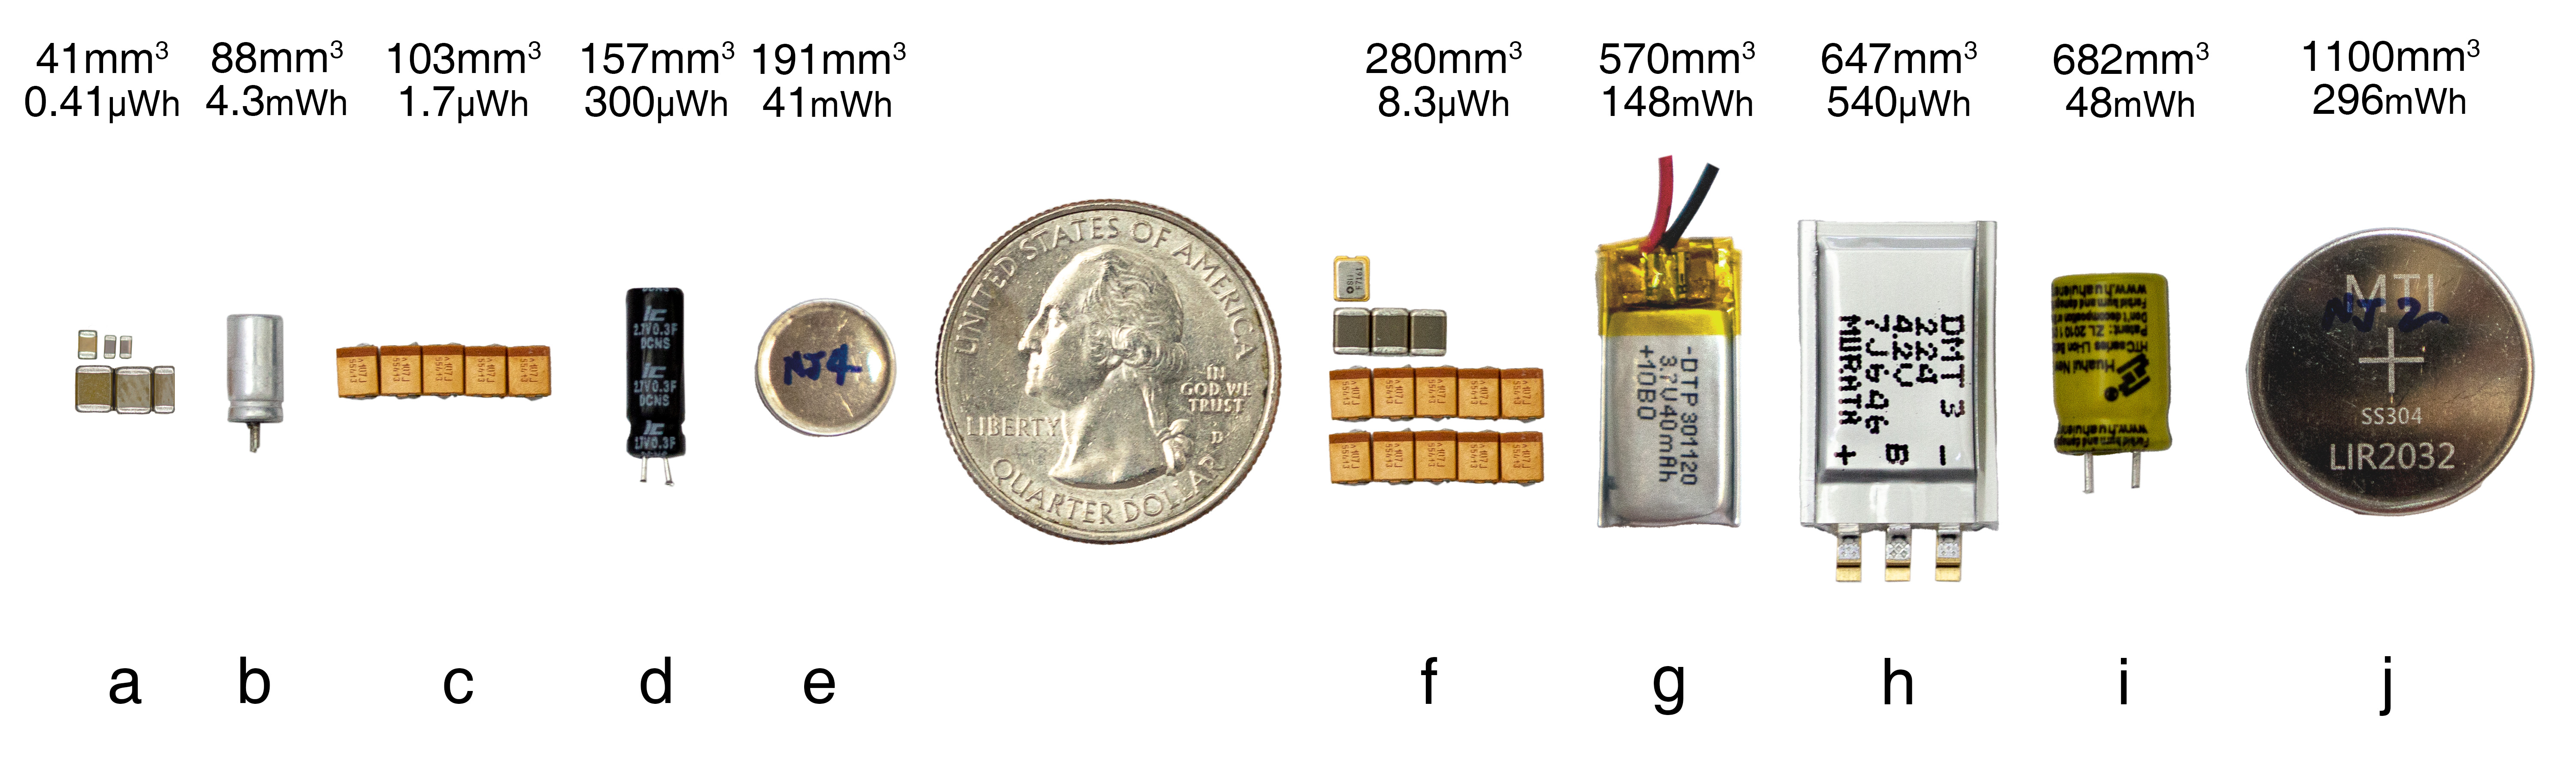
\includegraphics[width=\columnwidth]{figs/batteries/cap_lto_size_compare}
  \caption{
    A size comparison of energy storage methods including capacitors, supercapacitors, and batteries.
    \normalfont
    They are ordered left to right, by their
    (total) volume. Total volumes are listed above the respective device.
    Configuration
    \textbf{(a)}, \textbf{(c)} and \textbf{(e)} represent the energy storage configurations used
    in the Flicker platfrom with BLE and several sensors~\cite{hesterFlicker17}, the Solar Monjolo~\cite{campbellEnergy14} and the Capybara temperature
    monitor and alarm~\cite{colinReconfigurable18}, which have total
    capacitances and energy capacities of 119\si{\micro\farad} (0.41\si{\micro\Wh} at 5~V), 500\si{\micro\farad} (1.7\si{\micro\Wh} at 5~V)
    and 8.8\si{\milli\farad} (8.3\si{\micro\Wh} at 2.6~V), respectively. Capacitors
    \textbf{(d)}~\cite{illinoisCap} and \textbf{(f)}~\cite{murataCap} are large
    supercapacitors available on the Capybara platform and have the
    capacitances and energy capacities of 300\si{\milli\farad} (300\si{\micro\Wh} at 2.7\si{\volt}) and 220\si{\milli\farad}
    (540\si{\micro\Wh} at 4.2\si{\volt}) respectively.  While all pictured devices are
    similar in size and appearance, \textbf{(b)} and \textbf{(g)} are actually
    small LTO battery cells with 1.8\si{\milli\Ah} (4.3\si{\milli\Wh} at 2.4~V) and 20\si{\milli\Ah} (48\si{\milli\Wh}
    at 2.4\si{\volt}) capacity respectively~\cite{LTODatasheet2}. The LTO battery
    \textbf{(b)} is the second smallest of all configurations of energy storage
    presented here and also provides an order of magnitude more energy capacity
    compared to \textbf{(f)}, the largest supercapacitor presented.
  }
\end{definefigure}

\vspace{-6pt}
\noindent
\textbf{Bulky.}
As presented in \cref{tab:cost}, small batteries are 50-500x more dense than the supercapacitors and
three to five orders of magnitude more dense than ceramic and tantalum capacitors.
Even with an order of magnitude capacity reduction to achieve high cycle
lifetimes, batteries have a usable energy density of 5-50x greater than supercapacitors
of similar physical size.  The batteries shown \cref{fig:battery:sizes} are
as small as 88\,mm\textsuperscript{3}, and resemble small through-hole
capacitors. Battery \textbf{(b)} is smaller in volume than many of the capacitor
configurations presented in the literature, only outdone by systems like
Flicker \textbf{(a)} which store energy in only a few ceramic capacitors~\cite{hesterFlicker17},
and offers an order of
magnitude more energy storage than the largest supercapacitor presented. When
considering the size of other components in the system, most notably the
harvester (solar panel, thermocouple, or piezoelectric device), the combination
of large ICs, and large sensors like a PIR motion sensor, the size
of existing small rechargeable batteries is not significant.
Even the smallest energy harvesting sensor system to our knowledge,
the Michigan Micro Mote~\cite{lee13modular}, is on the
scale of a capacitor and utilizes a thin-film battery for energy storage.
\\

\placefigure[t]{fig:battery:sizes}

\vspace{-6pt}
\noindent
\textbf{Dangerous.} Traditional lithium metal batteries, such as
lithium cobalt chemistries, present risk of fire
and release of toxic gas under electrical and mechanical stress. Newer lithium-based
chemistries such as LTO and LiFePo\textsubscript{4} are considered much safer,
as they exhibit less thermal runaway under electrical, mechanical, and thermal
abuse~\cite{belharouakElectrochemistry11, larssonAbuse14}. Additionally,
unlike traditional lithium chemistries, LTO has been shown to not leak
any toxic and reactive gasses in the case of thermal abuse~\cite{belharouakElectrochemistry11}. They only release noble gasses.
While there is potential for danger under abuse conditions of these batteries,
there is ongoing research to create safer lithium batteries~\cite{larssonAbuse14}.

\begin{definetable*}{tab:cost}
        \begin{adjustbox}{width=0.95\textwidth}
    \begin{threeparttable}
    \centering
    \tiny
    \begin{tabular}{l | l | S[table-format=3.2,table-align-text-post = false] | S[table-format=3.3,table-align-text-post = false] | c | c | c | c | c | c | c}
      \multirow{2}{*}{Technology} & \multirow{2}{*}{Capacity} & {\multirow{2}{*}{\parbox{0.9cm}{\centering Volume\\(mm\textsuperscript{3})}}} & {\multirow{2}{*}{\parbox{1.6cm}{\centering Energy Density\\(Wh/L)}}} & \multirow{2}{*}{\parbox{2.2cm}{\centering Temperature Range\\(Charge/Discharge\,\textdegree C)}} & \multirow{2}{*}{ESR (\textOmega)} &  \multirow{2}{*}{\parbox{1.5cm}{\centering Self-Discharge\\(nA)}} &    \multicolumn{2}{c|}{Cycle Life (Cycles)} & \multicolumn{2}{c}{Cost (USD)}\\\cline{8-11}
                                    &                               &                   &                   &                                   &                           &                                       &  100\% DoD\,\tnote{l}& 10\% DoD\,\tnote{l}  & US\,\tnote{o}  & China\,\tnote{o}  \\\hline
            \multirow{2}{*}[0.6em]{MLCC} & 47\,\textmu F~\cite{ceramicDatasheet2}        & 1.28\,\tnote{a}   & 0.046\,\tnote{b}  & -55 - 125    & 0.001-0.1\,\tnote{g}      & <10\,\tnote{i}                        & Inf.\,\tnote{m}         & Inf.\,\tnote{m}   & 0.16          & 0.03  \\
                                    & 100\,\textmu F~\cite{ceramicDatasheet}           & 9.2\,\tnote{a}    & 0.013\,\tnote{b}  & -55 - 125      & 0.001-0.1\,\tnote{g}      & <10\,\tnote{i}                        & Inf.\,\tnote{m}         & Inf.\,\tnote{m}   & 0.31          & 0.04  \\
\multirow{2}{*}[0.6em]{Tantalum}    & 100\,\textmu F~\cite{tantalumDatasheet}           & 9.2\,\tnote{a}    & 0.013\,\tnote{b}  & -55 - 85      & 0.2                       & <10\,\tnote{i}                        & Inf.\,\tnote{m}         & Inf.\,\tnote{m}   & 0.28          & 0.17  \\
                                    & 220\,\textmu F~\cite{tantalumDatasheet}           & 9.2\,\tnote{a}    & 0.027\,\tnote{b}  & -55 - 85      & 0.07                      & <10\,\tnote{i}                        & Inf.\,\tnote{m}         & Inf.\,\tnote{m}   & 0.37          & 0.16  \\
\multirow{2}{*}[0.6em]{Supercapacitor}        & 7.5\,mF~\cite{seikoCap}       & 7.2               & 0.83\,\tnote{c}   & -30 - 70\,\tnote{d}               &    25                     &  {\textemdash}                        & >10000                  & \textemdash       & 2.42          & {\textemdash}     \\
                                    & 100\,mF~\cite{kemetCap}       & 1128              & 0.07\,\tnote{c}   & -25 - 70\,\tnote{d}               &   100                     & <10\,\tnote{j}                        & \textemdash             & \textemdash       & 1.10          & {\textemdash}     \\
                                    & 470\,mF~\cite{murataCap}      & 940               & 0.62\,\tnote{b}   & -40 - 70\,\tnote{d}               & 45                     & <1000                                 & 100000+/4\,yr~\cite{murataTech}\,\tnote{n} & \textemdash\,\tnote{n}   & 5.06          & 1.00  \\
\multirow{2}{*}[0.6em]{LiPo}        & 37\,mWh~\cite{10mahlipo}      & 297               & 125               & 0 - 40/-20 - 60\,\tnote{e}        &  {\textemdash}\,\tnote{k} & 30-100~\cite{zimmermanSelf04}         & 300-500                 & 10000+~\cite{guenaDepth06, millnerModeling10}
                                                                                                                                                                                                                                       &  {\textemdash}& 0.80  \\
                                    & 148\,mWh~\cite{lipoDatasheet} & 660               & 224               & 0 - 40/-20 - 60\,\tnote{e}        & 0.1                       & 120-400~\cite{zimmermanSelf04}        & 300                     & 10000+~\cite{guenaDepth06, millnerModeling10}
                                                                                                                                                                                                                                                                  & 4.50          & 0.51  \\
                                    & 148\,mWh~\cite{40mahlipo}     & 1005\,\tnote{a}   & 224               & 0 - 40/-20 - 60\,\tnote{e}        & 3                         & 120-400~\cite{zimmermanSelf04}        & 500                     & 10000+~\cite{guenaDepth06, millnerModeling10}
                                                                                                                                                                                                                                                                  & 1.62          & \textemdash \\
\multirow{2}{*}[0.6em]{LTO}         & 4.3\,mWh~\cite{LTODatasheet2} & 88                & 49                & -35 - 70\,\tnote{ef}              & 8                         &  {\textemdash}\,\tnote{k}             & 2000                    & 10000+~\cite{hallExperimental18}
                                                                                                                                                                                                                                                                  &  {\textemdash}& 1.01  \\
                                    & 60\,mWh~\cite{LTODatasheet,LTODatasheet2}  & 685  & 88                & 0 - 40/-20 - 60\,\tnote{ef}       & 2.4                       &  {\textemdash}\,\tnote{k}             & 2000                    & 10000+~\cite{hallExperimental18}
                                                                                                                                                                                                                                                                   & 6.75          & 1.01  \\
      LiFePo\textsubscript{4}                             & 96\,mWh~\cite{30mahlifepo}     & 1020             & 94                & 0 - 40/-20 - 60\,\tnote{e}        & 0.1  & 160~\cite{swierczynskiInvestigation14}& 2000~\cite{shenAdvanced13}
                                                                                                                                                                                                                                         & 30000+~\cite{wangCycle11,sarasketaCycle15,omarLithium14}
                                                                                                                                                                                                                                                   &  {\textemdash}& 0.95  \\
%\multirow{2}{*}[0.6em]{Li-Primary}  & 720\,mWh~\cite{primary2032}    & 1005\,\tnote{a}  & 716               & -30 - 60\,\tnote{e}               & {N/A\,\tnote{h}}          & 250                                   &N/A                      &  N/A              & 0.20          & 0.10  \\
%                                    & 4500\,mWh~\cite{primarycr123a} & 7830\,\tnote{a}  & 574               & -40 - 70\,\tnote{e}               & {N/A\,\tnote{h}}          & 1400                                  &N/A                      &  N/A              & 0.90          & 0.75  \\
%\multirow{2}{*}[0.6em]{Li-Thin Film}& 3.9\,mWh~\cite{thinDatasheet}  & 119              & 32.7              & -20 - 60\,\tnote{e}               & 80                        & 3.5                                   &4000                     &\textemdash        & 18.24         & {\textemdash}     \\
%                                    & 190\,\textmu Wh~\cite{thinDatasheet2} & 58        & 3.2               & -40 - 70\,\tnote{e}               & 2200                      & 0.2                                   &300                      &  5000             &  {\textemdash}& {\textemdash}     \\
   \end{tabular}
    \begin{tablenotes}[para]
        \item[a] Standard packages in order of increasing volume: 0603, 1206, 2032, CR123A.
        \item[b] Assumed 3\,V for energy calculation.
        \item[c] Assumed 2.4\,V, the max rated voltage, for energy calculation.
        \item[d] Supercapacitors experience higher ESR at lower temperatures and higher leakage at higher temperatures~\cite{murataTech}.\\
        \item[e] Lithium batteries experience higher ESR, higher leakage, lower capacity and shorter lifetimes at temperature extremes.\\
        \item[f] We believe these are produced by the same manufacturer, but have different suppliers and datasheets. We are skeptical of the wide temperature range.\\
        \item[g] ESR is frequency dependent.
        \item[h] ESR is conservatively calculated into rated capacity~\cite{feeneyDynamics14}.
        \item[i] Both tested and calculated from insulation resistance after absorption period.\\
        \item[j] Specification after 24\,h of charging.
        \item[k] We assume value to be similar to other Li cells, but cannot verify this assumption.\\
        \item[l] Measured to 80\% rated capacity.
        \item[m] We do not consider capacitor derating. With proper design principals these should be nearly infinite.\\
        \item[n] Supercapacitors are time rather than cycle limited. Assumes 3V, 20\,\textdegree C. No DoD dependence mentioned~\cite{murataTech}.
        \item[o] Prices are based on cheapest available equivalent part in quantities of 100.
    \end{tablenotes}
    \end{threeparttable}
        \end{adjustbox}
    \caption{A comparison of energy storage technologies that may be used on sensor nodes.
    \normalfont
    Data is based on specific components and their datasheets, and
    we attempt to choose representative components for each category, however
    some technologies such as supercapacitors are rapidly evolving. Other citations point to capabilities
    of the storage technologies not specified by their datasheets. We find that for
    most applications lithium-based batteries provide much higher energy density
    without reasonably impacting sensor lifetime, cost, or function.
    The minority of sensing applications, such as those operating at extreme
    temperatures, may require capacitors until battery technologies improve.}

\end{definetable*}